\section{About The Reflex Canvas \label{sec:about_canvas}}

\subsection{Saving And Loading Workflows}

In the course of your data reductions, it is likely that you will
customise the workflow for various data sets, even if this simply consists of 
editing the {\tt ROOT\_DATA\_DIR} to a different value for each data set. 
Whenever you modify a workflow in any way, you have the option of saving the 
modified version to an {\tt XML} file using {\tt File -> Export As} 
(which will also open a new workflow canvas corresponding to the saved file). 
The saved workflow may be opened in subsequent
{\tt Reflex} sessions using {\tt File -> Open}. Saving the workflow in the
default format (.kar) is only advised if you do not plan to use the workflow
in other computer.

\subsection{Buttons}  
         
At the top of the {\tt Reflex} canvas are a set of buttons which have the following useful functions:
\begin{itemize}
\item{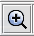
\includegraphics[width=0.5cm,height=0.5cm]{reflex_zoom_in_button.png} - Zoom in.}
\item{
\includegraphics[width=0.5cm,height=0.5cm]{reflex_zoom_reset_button.png} - Reset the zoom to 100\%.}
\item{
\includegraphics[width=0.5cm,height=0.5cm]{reflex_zoom_to_fit_button.png} - Zoom the workflow to fit the current window size (Recommended).}
\item{
\includegraphics[width=0.5cm,height=0.5cm]{reflex_zoom_out_button.png} - Zoom out.}
\item{
\includegraphics[width=0.5cm,height=0.5cm]{reflex_run_button.png} - Run (or resume) the workflow.}
\item{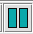
\includegraphics[width=0.5cm,height=0.5cm]{reflex_pause_button.png} - Pause the workflow execution.}
\item{
\includegraphics[width=0.5cm,height=0.5cm]{reflex_stop_button.png} - Stop the workflow execution.}
\end{itemize}
The remainder of the buttons (not shown here) are not relevant to the 
workflow execution.

\subsection{Workflow States}

A workflow may only be in one of three states: executing, paused, or stopped.
 These states are indicated by the yellow highlighting of the

\includegraphics[width=0.5cm,height=0.5cm]{reflex_run_button.png},
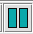
\includegraphics[width=0.5cm,height=0.5cm]{reflex_pause_button.png},
and 
\includegraphics[width=0.5cm,height=0.5cm]{reflex_stop_button.png}
buttons, respectively. A workflow is executed by clicking the

\includegraphics[width=0.5cm,height=0.5cm]{reflex_run_button.png} button. 
Subsequently the workflow and any running
pipeline recipe may be stopped immediately by clicking the

\includegraphics[width=0.5cm,height=0.5cm]{reflex_stop_button.png}
button, or the workflow may be paused by clicking the 
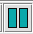
\includegraphics[width=0.5cm,height=0.5cm]{reflex_pause_button.png} button which
will allow the current actor/recipe to finish execution before the workflow is 
actually paused. Note that after clicking the
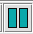
\includegraphics[width=0.5cm,height=0.5cm]{reflex_pause_button.png} button, 
it is possible that more than one actor is executed, since this behaviour 
depends on the workflow scheduling. For instance, if there are two actors in 
parallel, and you pause the workflow while one is being executed, then both
of them will be executed before the workflow is actually paused. After pausing,
the workflow may be resumed by clicking the

\includegraphics[width=0.5cm,height=0.5cm]{reflex_run_button.png} button again.

\subsection{The Runtime Window}

You may find the runtime window a useful aid in monitoring the
reduction progress of your data. This window may be started by
clicking {\tt Workflow -> Runtime Window} from the {\tt Reflex} canvas
menu. You will notice that on the left-hand side the runtime window
has buttons allowing the control of the workflow (\fbox{\tt Go},
\fbox{\tt Pause}, \fbox{\tt Resume}, \fbox{\tt Stop}) and text boxes
for controlling workflow parameters such as the working data directory
etc.

On the right-hand side of the runtime window is a text box with the
title ``Recipe Status'' which lists the current status of each
pipeline recipe and the reduction status of each DataSet. A recipe may
have the following status values:
\begin{itemize}
\item{{\tt Not Running} - The recipe has not yet been run for any DataSet so far.}
\item{{\tt Executing} - The recipe is currently executing for a DataSet.}
\item{{\tt Done} - The last execution of the pipeline recipe was successful.}
\item{{\tt Failed} - The recipe failed on the last DataSet.}
\item{{\tt Skip} - The recipe was skipped for the last DataSet.}
\item{{\tt Disabled} - The recipe was disabled for the last DataSet.}
\item{{\tt Stopped} - The workflow was stopped during the reduction of a DataSet.}
\end{itemize}

Below the list of recipe status values is a detailed list of input and
output files used for each DataSet within each recipe execution. This
information is sometimes very useful for the user who wants to know
exactly which files were used as input for a particular DataSet for a
given pipeline recipe, and where the relevant output files were
written.
